% !TEX TS-program = pdflatex
% !TEX encoding = UTF-8 Unicodeo
\documentclass[3p,times]{elsarticle}

%=============================================================================
%==========  A L L    I N C L U D E S
%%%%%%%%%% PACKAGES %%%%%%%%%% 
%\usepackage[utf8x]{inputenc}
\usepackage{array}
\usepackage{color} 
\usepackage{tabularx}
\usepackage{graphicx} 
\usepackage{amsmath}
\usepackage{amssymb}
\usepackage{amsfonts}	
\usepackage{moreverb}
\usepackage{dsfont}
\usepackage{tipa}
\usepackage{upgreek}
%\usepackage{grffile}
\usepackage{bm}
\usepackage{multirow}
\usepackage{soul}
\usepackage{ textcomp }
\usepackage{relsize} % e.g. used for \mathsmaller

\renewcommand{\tabularxcolumn}[1]{m{#1}}
\newcommand\BibTeX{{\rmfamily B\kern-.05em \textsc{i\kern-.025em b}\kern-.08em
T\kern-.1667em\lower.7ex\hbox{E}\kern-.125emX}}


%%%%%%%%%% PACKAGES %%%%%%%%%%

\renewcommand{\tabularxcolumn}[1]{m{#1}}

% To have colored cited papers, hyperlinked to the 
% bibiography, help to know if papers are not cited
% but in the bibliography still
\usepackage{hyperref} 
\hypersetup{
    colorlinks=true,                          
    linkcolor=blue, % Couleur des liens internes
    citecolor=red, % Couleur des num�ros de la biblio dans le corps
    urlcolor=blue  } % Couleur des url
%\usepackage[hyperpageref]{backref} 
%usepackage[square,numbers]{natbib}
%\RequirePackage[hyperpageref]{backref}
%\backreffrench
%\renewcommand*{\backref}[1]{}  % Disable standard
%\renewcommand*{\backrefalt}[4]{% Detailed backref
 %\ifcase #1 %
 %\relax%(Not cited.)%
  %\or
%% (Cit\'e page~#2.)%
 %(Cited page~#2.)%
 %\else
 %%(Cit\'e pages~#2.) 
 %(Cited page~#2.)%
 %\fi}

\setlength{\oddsidemargin}{.5cm} \setlength{\evensidemargin}{.5cm}
\setlength{\textwidth}{15cm} \setlength{\textheight}{21.0cm}
\setlength{\topmargin}{0in}

%%%%%%%% NEW COMMANDS %%%%%%%%
\newcommand{\pd}{\mathcal{\partial}}
\newcommand{\ce}{{\varepsilon}}
\newcommand{\xx}{{\boldsymbol{x}}}
\newcommand{\yy}{{\boldsymbol{y}}}
\newcommand{\zz}{{\boldsymbol{z}}}
\newcommand{\x}{\mbf{x}}
\newcommand{\y}{\mbf{y}}
\newcommand{\Th}{\mathcal{T}_h}				%mesh notation
\newcommand{\nij}{\mathbf{n}_{ij}}				%outward unit normal to S_ij
\newcommand{\Eel}{\mathcal{E}_{el} }			%indices set of the real cells
\newcommand{\Ebd}{\mathcal{E}_{bd} }			%indices set of the virtual cells
\newcommand{\tEel}{\widetilde{\mathcal{E}_{el}}}	%indices set of the real and virtual cells
\newcommand{\Epc}{\mathcal{E}_{pc} }			%indices set of problematic cells
\newcommand{\Unui}{\underline{\nu}(i)}		%indices set of cells linked to K_i by a side
\newcommand{\Onui}{\overline{\nu}(i)}			%indices set of every cells linked to K_i
\newcommand{\urec}{\widetilde u}				%polynomial rec sur K
\newcommand{\Urec}{\widetilde U}				%polynomial rec sur K
\newcommand{\R}[2]{{\mc{R}}^{\{#1,#2\}}} %NEEDED FOR POLY REC ..
\newcommand{\CPD}{\textsf{CellPD}}
%\newcommand{\un}{\textrm{1}}
\newcommand{\un}{1 \hskip -3pt \textrm{I}}
\newcommand{\Deg}[1]{ \mathsf{d}_{#1} }
\newcommand{\EPD}{\textsf{EdgePD}}
\newcommand{\FPD}{\textsf{FacePD}}
\newcommand{\EPDMeth}[1]{$\mathsf{EPD}_{\mathsf{#1}}$}
\newcommand{\mc}[1]{\mathcal{#1}}			% Simplification of usefull calligraphies
\newcommand{\mbb}[1]{\mathbb{#1}}			%
\newcommand{\mbf}[1]{\mathbf{#1}}			%
\newcommand{\msf}[1]{\mathsf{#1}}		       %
\newcommand{\mait}[1]{\mathit{#1}}			%
\newcommand{\mfrk}[1]{\mathfrak{#1}}		%
\newcommand{\tbf}[1]{\textbf{#1}}				%
\newcommand{\tsf}[1]{\textsf{#1}}				%
\newcommand{\tit}[1]{\textit{#1}}					%
\newcommand{\trm}[1]{\textrm{#1}}					%
\newcommand{\noi}{\noindent}
\newcommand{\Frac}{\displaystyle\frac}
\newcommand{\Int}{\displaystyle\int}
\newcommand{\Sum}{\displaystyle\sum}
\newcommand{\Bigcup}{\displaystyle\bigcup}
\newcommand{\Max}{\displaystyle\max}
\newcommand{\Min}{\displaystyle\min}
\newcommand{\Eq}[1]{equation {(\ref{#1})}}
\newcommand{\Q}{\mathbf{Q}}
\renewcommand{\S}{\mathbf{S}}
\renewcommand{\u}{\mathbf{u}}
\newcommand{\w}{\mathbf{w}}
\newcommand{\m}{\mathbf{m}}
\newcommand{\q}{\mathbf{q}}
\newcommand{\F}{\mathbf{F}}
\newcommand{\f}{\mathbf{f}}
\newcommand{\g}{\mathbf{g}}
\newcommand{\h}{\mathbf{h}}

\renewcommand{\v}{\mathbf{v}}
\newcommand{\B}{\mathbf{B}}
\newcommand{\Ell}{\mathcal{L}}
\newcommand{\emm}{m}
\newcommand{\dxx}[1]{ \partial_{xx} #1 }
\newcommand{\dyy}[1]{ \partial_{yy} #1 }
\newcommand{\dzz}[1]{ \partial_{zz} #1 }
\newcommand{\HRule}[1]{ {\centering \rule{#1\linewidth}{0.2mm}} }
\newcommand{\DMPutwo}{$[\text{DMP}\!\to\!u2]$}
\newcommand{\PADDMPutwo}{$[\text{PAD}\!\to\!\text{DMP}\!\to\!u2]$}
\newcommand{\red}[1]{{\color{red} #1}}
\newcommand{\blue}[1]{{\color{blue} #1}}
\newcommand{\mygreen}{\textcolor[rgb]{0.0,0.60,0.}}
\newcommand{\myorange}{\textcolor[rgb]{0.6,0.0,0.}}
\newcommand{\oz}[1]{ \textcolor{red}   {\texttt{\textbf{OZ: #1}}} }
\newcommand{\rmd}{{\rm d}}


% Michael DUMBSER Aliases
\newcommand{\CK}{Cauchy-Kovalewski }
\newcommand{\CPU}{\textnormal{CPU}}
\newcommand{\p}{\textnormal{P}}
\newcommand{\PM}{\mathbb{P}_M}
\newcommand{\PNPM}{\mathbb{P}_N\mathbb{P}_M}
\newcommand{\PNM}{\mathbb{P}_N\mathbb{P}_M}
\newcommand{\PMM}{\mathbb{P}_N\mathbb{P}_N}
\newcommand{\PzM}{\mathbb{P}_0\mathbb{P}_M} 
\newcommand{\PMPM}{\mathbb{P}_M\mathbb{P}_M}
\newcommand{\dt}{\frac{\partial}{\partial t}}
\newcommand{\dx}{\frac{\partial}{\partial x}}
\newcommand{\dy}{\frac{\partial}{\partial y}}
\newcommand{\dz}{\frac{\partial}{\partial z}}
\newcommand{\Path}{\mathbf{\Psi}}
\newcommand{\dtau}{\frac{\partial}{\partial \tau}}
\newcommand{\dxi}{\frac{\partial}{\partial \xi}}
\newcommand{\deta}{\frac{\partial}{\partial \eta}}
\newcommand{\dzeta}{\frac{\partial}{\partial \zeta}}
\newcommand{\tens}[1]{\underline{\underline{#1}}}
%\newcommand{\tens}[1]{{\mathbf{#1}}}
\newcommand{\K}{\tens{K}}
\newcommand{\M}{\tens{M}}
\newcommand{\Roe}{\textnormal{Roe}}
\newcommand{\HLL}{\textnormal{HLL}}
\newcommand{\U}{\mathcal{U}}
\newcommand{\G}{\mathbf{G}}
\newcommand{\A}{\AAA}
\newcommand{\Fd}{\mathcal{F}}
\newcommand{\Gd}{\mathcal{G}}
\newcommand{\Hd}{\mathcal{H}}
\newcommand{\Sd}{\mathcal{S}}
\newcommand{\tot}{\textnormal{tot}}
\newcommand{\CFL}{\textnormal{CFL}}
\newcommand{\for}{\textnormal{for}}
\newcommand{\nn}{n+\frac{1}{2}}
\newcommand{\jj}{j+\frac{1}{2}}
\newcommand{\Qi}{\mathbf{Q}_i^n} 
\newcommand{\Qj}{\mathbf{Q}_j^n} 
\newcommand{\Qjj}{\mathbf{Q}_{j+\frac{1}{2}}^{n+\frac{1}{2}}} 
\newcommand{\Aip}{V_i^+} 
\newcommand{\Aim}{V_i^-} 
\newcommand{\Ajp}{V_j^+} 
\newcommand{\Ajm}{V_j^-} 
\newcommand{\Aom}{V_1^-} 
\newcommand{\Atm}{V_2^-} 
\newcommand{\Ahm}{V_3^-} 
\newcommand{\AT}{\left|T_i\right|}
\newcommand{\halb}{\frac{1}{2}}
\newcommand{\FQi}{\tens{\mathbf{F}}\left(\Qi\right)}
\newcommand{\FQj}{\tens{\mathbf{F}}\left(\Qj\right)}
\newcommand{\FQjj}{\tens{\mathbf{F}}\left(\Qjj\right)}
\newcommand{\nj}{\vec n_j}
\newcommand{\FORCE}{\textnormal{FORCE}}
\newcommand{\GFORCE}{\textnormal{GFORCEN}}
\newcommand{\LF}{\textnormal{LF}'}
\newcommand{\LW}{\textnormal{LW}'}
\newcommand{\WL}{\mathcal{W}_h^-}
\newcommand{\WR}{\mathcal{W}_h^+}
\newcommand{\nur}{\boldsymbol{\nu}^\textbf{r} }
\newcommand{\nuf}{\boldsymbol{\nu}^{\boldsymbol{\phi}} }
\newcommand{\nut}{\boldsymbol{\nu}^{\boldsymbol{\theta}} }
\newcommand{\ar}{\phi_1\rho_1}
\newcommand{\arr}{\phi_2\rho_2}
\newcommand{\ur}{u_1^r}
\newcommand{\uf}{u_1^{\phi}}
\newcommand{\ut}{u_1^{\theta}}
\newcommand{\urr}{u_2^r}
\newcommand{\uff}{u_2^{\phi}}
\newcommand{\utt}{u_2^{\theta}}
\newcommand{\ub}{\textbf{u}_\textbf{1}}
\newcommand{\ubb}{\textbf{u}_\textbf{2}}
\newcommand{\RoeMat}{{\tilde A}_{\Path}^G} 
\newcommand{\bdm}{\begin{displaymath}}
\newcommand{\edm}{\end{displaymath}}

\newcommand{\bea}{\begin{eqnarray} }
\newcommand{\eea}{\end{eqnarray} }

\newcommand{\apriori}{\textit{a priori} }
\newcommand{\aposteriori}{\textit{a posteriori} }

\newcommand{\dev}{\textnormal{dev}} 

\newcommand{\AAA}{{\boldsymbol{A}}}
\newcommand{\aaa}{{\boldsymbol{a}}}
\newcommand{\DD}{{\mathbf{D}}}
\newcommand{\HH}{{\mathbf{H}}}
\newcommand{\sfA}{{\mathsf{A}}}
\newcommand{\sfB}{{\mathsf{B}}}
\newcommand{\GG}{{\boldsymbol{G}}}
\newcommand{\rr}{{\mathbf{r}}}
\newcommand{\ee}{{\mathbf{e}}}
\newcommand{\bb}{{\mathbf{b}}}
\newcommand{\hh}{{\mathbf{h}}}
\newcommand{\dd}{{\mathbf{d}}}
\newcommand{\vv}{{\boldsymbol{v}}}
\newcommand{\uu}{{\mathbf{u}}}
\newcommand{\mcE}{{\mathcal{E}}}
\newcommand{\calI}{\mathcal{I}}
\newcommand{\EE}{{\mathbf{E}}}
\newcommand{\BB}{{\mathbf{B}}}

\newcommand{\FF}{{\boldsymbol{F}}}
\newcommand{\II}{{\mathbf{I}}}
\newcommand{\JJ}{{\mathbf{J}}}
\newcommand{\QQ}{{\mathbf{Q}}}
\newcommand{\QV}{{\mathbf{V}}}
\newcommand{\PP}{{\mathbf{P}}}
%\newcommand{\SS}{{\boldsymbol{S}}}
\newcommand{\WW}{{\mathbf{W}}}
\newcommand{\ww}{{\bm{w}}}
\newcommand{\wbf}{{\mathbf{w}}}
\newcommand{\pp}{{\mathbf{p}}}
\newcommand{\qq}{{\mathbf{q}}}

\newcommand{\Id}{{\mathbf{I}}}
\newcommand{\tr}{\textnormal{tr}}
\newcommand{\BS}{{\boldsymbol{\sigma}}}
\renewcommand{\Re}{\textnormal{Re}}
\newcommand{\transpose}{{\rm {\mathsmaller T}}}



%%%%%%%%%%%%%%%%%%%%%%%%%%%%%%%%%%%%%%%%%%%%%%%%%%%%%
%%%%%%%%%%%%%%%%%%%%%%%%%%%%%%%%%%%%%%%%%%%%%%%%%%%%%
%%%%%%%%%%%%%%%%%%%%%%%%%%%%%%%%%%%%%%%%%%%%%%%%%%%%%
% DOC BEGINNING

\newfont{\numerikEleven}{ecrm1000}
\newfont{\numerikTen}{cmss10}
\newfont{\numerikNine}{cmss9}
\newfont{\numerikEight}{cmss8}

%=========================================================================

\journal{Journal of Dead End Ideas}

\begin{document} 
%!=========================================================================
%!
%!      F R O N T    M A T T E R 
%!
\begin{frontmatter}
%-------------------------------------------------------
% TITLE
\title{Modeling of wavefields in saturated elastic porous medium based on thermodynamically compatible system theory for multiphase mixture } 
%-------------------------------------------------------
%-------------------------------------------------------
% AUTHORS
\author[NSC,NSU]{Evgeniy Romenski}
\ead{evrom@math.nsc.ru}

\author[ICMMG]{Galina Reshetova}
\ead{kgv@nmsf.sscc.ru}
 
\author[IMT,NSC]{Ilya Peshkov}
\ead{peshkov@math.nsc.ru}
\cortext[cor1]{Corresponding author}

\author[UniTN]{Michael Dumbser$^{*}$}
\ead{michael.dumbser@unitn.it}

%\cortext[cor1]{{Ilya Peshkov is on leave from Sobolev Institute of Mathematics , 4 Acad. Koptyug Avenue, 630090 Novosibirsk, Russia}}


%-------------------------------------------------------
% INSTITUTIONS
\address[NSC]{{Sobolev Institute of Mathematics, 4 Acad. Koptyug Avenue, 630090 Novosibirsk, Russia}}
\address[ICMMG]{{Institute of Computational Mathematics and Mathematical Geophysics, 6 Pr. Akademika Lavrentjeva, 630090 Novosibirsk, Russia}}
\address[NSU]{{Novosibirsk State University, 2 Pirogova Str., 630090 Novosibirsk, Russia}}
\address[IMT]{{Institut de Math\'{e}matiques de Toulouse, Universit\'{e} Toulouse III, F-31062 Toulouse, France.}}
\address[UniTN]{Department of Civil, Environmental and Mechanical Engineering, 
University of Trento, Via Mesiano 77, 38123 Trento, Italy.} 
%-------------------------------------------------------

%-------------------------------------------------------
% ABSTRACT
\begin{abstract} \color[rgb]{0,0,0}
A multiphase model and its application to the wavefields numerical simulation are discussed for the description of compressible fluid flow in elastic porous medium. The proposed model is an extension of the unified model of continuum mechanics proposed in [1,2]. The derivation is based on the theory of thermodynamically compatible systems and on the model of nonlinear elastoplasticity combined with the multiphase compressible flow model [3]. The governing equations of the model include the phase mass conservation laws, total momentum conservation law, equation for relative velocities of phases, equations for deformation gradient of the medium and balance equation for porosity. They form a hyperbolic system of conservation form equations and satisfy fundamental laws of thermodynamics. Two types of phase interaction are introduced in the model: phase pressure relaxation to the common value and interfacial friction. The inelastic deformation also can be accounted by the source terms in the equation for the deformation gradient. The formulated model can be used for study a compressible fluid flow in a deformable elastoplastic porous medium in general, and for modeling wave propagation in a saturated porous medium in particular. 

The governing equations for small amplitude wave propagation in the uniform porous medium saturated with a single fluid medium are derived. They form the first-order hyperbolic PDE system written in terms of stress and velocities and, like in Biot’s model, predict three type of waves: fast and slow longitudinal waves and shear wave existing in the fluid-saturated porous medium. For the numerical solution of these equations an efficient numerical method based on staggered-grid finite difference scheme is used. The solution of some numerical test problems is presented and discussed.

\end{abstract}
%-------------------------------------------------------

%-------------------------------------------------------
% KEY WORDS
\begin{keyword}
 %symmetric hyperbolic thermodynamically compatible systems (HTC) \sep 
 %unified first order hyperbolic model of continuum mechanics  \sep 
 %non-Newtonian flows \sep
 %viscoplastic and yield stress fluids \sep
 %Bingham fluids \sep
 %arbitrary high-order ADER Discontinuous Galerkin schemes \sep 
 %path-conservative methods and stiff source terms  
%
%\PACS 
%\MSC
\end{keyword}
%-------------------------------------------------------
\end{frontmatter}
%!===================================================Partially======================

%-----------------------------------
% CONTENTS
%  This will deseapear in the submitted version
%\tableofcontents
%------------------------------------

%=========================================================================
%==========         I N T R O D U C T I O N
% 
\section{Introduction} \label{sec:introduction}
%
The modeling of fluid flows in porous media is of permanent interest in many geophysical and industrial applications. The starting point of research developments in this field was the series of pioneering work of Bio \cite{Bio}-\cite{Bio}, in which a model of elastic wave propagation in saturated porous media modeling was proposed. Some modification and generalization of the model have been done in the past (see \cite{} and references therein) and at present Biot's approach is the commonly accepted and widely used in geophysical community. Nevertheless, many actual technological and scientific problems such as geothermal energy extraction, CO2 storage, hydraulic fracturing require a development of new advanced models and methods. 

For the development of the nonlinear, temperature dependent processes in porous media the methods of continuum mechanics, and in particular multiphase theories can be succesfully applied. 
%A comprehensive review of the past and existing aproaches in the development of porous media %models one can find in the book \cite{Nikolaevsky}
Most consistently the two-phase approach has been inplemented by K. Wilmanski in \cite{Wilmanski1998}-\cite{Wilmanski2006} (see also references therin). In particular in the review paper \cite{Wilmanski2006}, the structure of Biot's poroelastic model is analysed and its admissibility within the fundamental principles of continuum mechanics is discussed. 

In recent years, a significant attention is paid for the modeling of large deformations of the saturated porous media and application to different areas, and in particularly in medicine, see
for example \cite{Khoei2011}, \cite{Rohan2017}, \cite{Pesavento2017}.
It is necessary to mention a model of the saturated porous medium proposed by Dorovsky \cite{Dorovsky} in which a significant attention is paid to thermodynamic consistency of the model and hyperbolicity of the governing equations. 
Nevertheless, there is still no a conventional thermodynamically consistent formulation of multiphase mixture flow in the  deforming porous medium subject finite deformatons. 

In the paper we apply a powerful method of the design of new models of complex continuum media  based on the thermodynamically compatible system theory and allowing the development of mathematically correct models satisfying fundamental laws of irreversible thermodynamics. 
In series of papers \cite{} - \cite{} it was formulated a class of Symmetric Hyperbolic Thermodynamically Compatible (SHTC) systems, which is able to describe all the known classical equations of continuum mechanics and electrodynamics (fluid mechanics, solid mechanics, electrodynamics, magneto hydrodynamics) in one single mathematical model, including both, advective and dissipative processes. All SHTC systems have nice mathematical properties: symmetric hyperbolicity in sense of Friedrichs and a conservative form of the equations. Solutions of the governing PDE satisfy all fundamental laws of non-equilibrium irreversible thermodynamics, namely the conservation of total energy (first law) and the non-decrease of physical entropy (second law). 

The SHTC system theory is based on the first principles, the governing PDEs for a very wide class of physical processes can be derived as the Euler-Lagrange equation from Hamilton’s principle
of stationary action. Then by the transformation of obtained Lagrangian equations to Eulerean equation and variables one can derive the master system in terms of generating thermodynamic potential and generating variables. This master system can be used for the design of well-posed model of physical process physical process of interest to us by the specific choice of potential and identifying generating variables with physical ones. The SHTC system approach has been succefully applied, for example, for the design of compressible multiphase flow  \cite{}, \cite{}. 
Recently unified SHTC model of Newtonian continuum mechanics has been developed describing at the same time the dynamics of elastoplastic solids as well as and SHTC multiphase flow model and is also belongs to the SHTC equations class. The interface friction between liquid and solid phases and shear stress relaxation are implemented in the model in accordance with laws of thermodynamics. The latter allows to account the dependence of elastic moduli on frequency in the time domain and apply a difference numerical methods to study wave propagation problems.  

The rest of the paper is organizet as follows. Section 2 brefly describes governing PDEs for unified model of continuum and for two-phase compressible fluid model. Then, by combining te above models, the governing master SHTC system for two-phase solid-fluid medium is formulated.
In Section 3 on the base of the presented model, the governing equations are derived for small amplitude wave propagation in the stationary saturated porous medium. In Section 4 we derive dispersion relation for the derived acoustic equations and study the properties of wavefields. Section 4 discuses differences and similatiries of Biot's and presented model.
In Section 5 an efficient numerical difference method for small amplitude wave propagation is presented and some numerical results are presented.         




%
%In \cite{HPR2016,DPRZ2016}, a unified first order hyperbolic formulation for 
%continuum mechanics was proposed. It was further extended 
%in~\cite{HPR2016elmag} to deal with coupling of matter and electro-magnetic 
%fields. It was shown 
%in~\cite{HPR2016,DPRZ2016,BartonRom2010,Pesh2010,BartonRom2012} that such a 
%unified formulation of continuum mechanics contains Newtonian fluids and 
%elastic and elastoplastic solids as particular cases. 


\section{System of governing PDEs for poroelastic medium}

The development of poroelastic model, the governing equations of which form the symmetric 
hyperbolic thermodynamically compatible (SHTC) system is based on the coupling of 
the unified thermodynamically compatible continuum model formulated in \cite{Dumbser2016} and two-phase compressible fluid model \cite{Romenski2010}. 

\subsection{SHTC governing equations of the unified solid-fluid model}

The PDE system of the unified model for deforming continuum reads as 
\begin{eqnarray} \label{eqn.HPR}
	&&\displaystyle\frac{\partial \rho v^i}{\partial t}+\frac{\partial 
		\left(\rho v^i v^k + p \delta_{ik} - \sigma_{ik} \right)}{\partial x_k}=0, 
	\label{eqn.momentum}\\[2mm]
	&& \frac{\partial \rho}{\partial t}+\frac{\partial \rho v^k}{\partial 
	x_k}=0,\label{eqn.conti}\\[2mm]
	&&\displaystyle\frac{\partial A_{i k}}{\partial t}+\frac{\partial A_{im} 
		v^m}{\partial x_k}+v^j\left(\frac{\partial A_{ik}}{\partial 
		x_j}-\frac{\partial A_{ij}}{\partial x_k}\right)
	=-\dfrac{ \psi_{ik} }{\theta},\label{eqn.deformation}\\[2mm]
	&&\displaystyle\frac{\partial \rho s}{\partial t}+\frac{\partial \rho 
		s v^k }{\partial x_k}=\dfrac{\rho}{\theta T} 
	\psi_{ik} \psi_{ik} \geq0, 
	\label{eqn.entropy}
\end{eqnarray}
Here \eqref{eqn.conti} is the mass coservation law, \eqref{eqn.momentum} is the momentum conservation law, \eqref{eqn.deformation} is the evolution of distortion tensor, \eqref{eqn.entropy} is the entropy balance law.
As the independent set of the parameters of state we take:
velocities $v^k$, mass density $\rho$, distortion $A_{ik}$, and entropy $s$.
Additional parameters of the medium are presented in the above system: the pressure $p$, shear stress $\sigma_{ik}$, and temperature $T$. They are connected with the density, distorsion and entropy via specific total energy $E(\bf{v},\rho,s,\bf{A})$:
\begin{align}
p=\rho^2\frac{\partial E}{\partial \rho}, \quad 
\sigma_{ij}=-\rho A_{ki}\frac{\partial E}{\partial A_{kj}}, \quad 
T=\frac{\partial E}{\partial s}.
\end{align}
The source term in the equation for distortion characterizes the rate of inelastic deformation,
where ${\bf{\psi}}=\frac{\partial E}{\partial {\bf{A}}}$.
The parameter $\theta(\tau)$ depends on the shear stress relaxation time $\tau$ which can vary from $\infty$ (elastic medium) to $0$ (inviscid fluid).

The closure of the model requires to define the dependence of the energy $E$ and parameter $\theta$ on the parameters of state.
We take the energy in the form
\begin{align}
E=E_1(\rho,s)+E_2(\rho,s,{\bf A})+E_3({\bf v}), \label{energy}
\end{align}
where $E_3=\frac{1}{2}v^iv^i$ is the specific kinetic energy,
$E_1$ is the "hydrodynamic" part correponding to the energy of the volume deformations only,
and $E_2$ is the energy of shear strain.
In order to provide zero trace of shear stress $\tr ({\bf \sigma})=0$, we take $E_2$ depending on ${\bf A}$ via the normalized strain tensor ${\bf g}={\bf a}^T{\bf a}$, where ${\bf a}={\bf A}/(\det {\bf A})^{1/3}$. It gives us ${\bf g}={\bf G}/(\det{\bf G})^{1/3}$, where ${\bf G}={\bf A}^T{\bf A}$. Then the energy of shear stress can be defined as an elastic energy in a separable form \cite{Gavrilyk} 
\begin{align}
E_2=\frac{1}{8}c_s^2\left(\tr({{\bf g^2}})-3\right),
\end{align}
where $c_s$ is the shear wave of sound at the reference conditions.

With the use of above definition we can compute
the derivative of $E$ with respect to $A$
\begin{align} \label{EderivA}
\frac{\partial E}{\partial A}=\frac{\partial E_2}{\partial A}=-F^T\frac{\sigma}{\rho}=
\frac{c_s^2}{2} F^T \left({\bf g^2}-\frac{\tr({{\bf g^2}})}{3} {\bf I}. \right),
\end{align}
where $F=A^{-1}$.
Then the shear stress reads as
\begin{align}
{\bf \sigma}=-\rho \frac{c_s^2}{2}\left({\bf g^2}-\frac{\tr({{\bf g^2}})}{3} {\bf I}. \right), \quad  \tr({\bf \sigma})=0.
\end{align} 

Coefficient $\theta$ is a function of the parameters of state and should be taken in the form 
\begin{align}
\theta = \tau \theta_0(\rho,T,Y) \textgreater 0,
\end{align}
where $Y=\frac{1}{2}\sqrt{tr(\sigma^2)}$ is the intensity of shear stress,
$\tau$ is the characteristic shear stress relaxation time (for elastic material $\tau=\infty$).

The source term in the equation for distortion produces the nonnegative entropy production source term in \eqref{eqn.entropy}. 
It is important to note that for system \eqref{eqn.HPR}-\eqref{eqn.entropy} the additional energy conservation law holds:
\begin{align} \label{eqn.energy}
\displaystyle\frac{\partial \rho E}{\partial t}+
\frac{\partial \left(\rho  v^k E +v^i(p \delta_{ik}-\sigma_{ik}) \right)}{\partial x_k}=0.
\end{align}

\subsection{SHTC governing equations of two-phase compressible fluid flow model}

In the two-phase compressible fluid model the flow in general is considered as a mixture of two immisible constituents with thier own parameters of state. Thus, the general model should take into account the difference between velocities, pressures and tempertures of phases. That means that if we consider the velosity, density, and entropy as the basic parameters of state, then they are different for each phase. In our consideration we restrict ourselves by the single entropy approximation which is suitable for small variations of phase temperatures \cite{Romenski2015}  

The SHTC system for two-phase compressibe flow with the single entropy approximation \cite{Romenski2010} reads as follows:
\begin{eqnarray}\label{eqn.HPRFF}
&&\displaystyle\frac{\partial \rho v^i}{\partial t}+\frac{\partial 
	(\rho v^i v^k + p \delta_{ik} + w^iE_{w^k} )}{\partial x_k}=0, 
\label{eqn.momentumFF}\\[2mm]
&& \frac{\partial \rho}{\partial t}+\frac{\partial \rho v^k}{\partial 
	x_k}=0,\label{eqn.contiFF}\\[2mm]
&& \frac{\partial \rho c_1}{\partial t}+\frac{(\partial \rho c_1 v^k+E_{w_k})}{\partial 
	x_k}=0,\label{eqn.contiFF}\\[2mm]
&&\displaystyle\frac{\partial w^k}{\partial t}+\frac{(w^lv^l+E_c)}{\partial x_k}+\varepsilon_{klj}v^l\omega_j (=\varepsilon_{jmn}\left(\frac{\partial w^m}{\partial x_n}-\frac{\partial w^n}{\partial x_m}\right))=-\dfrac{ \lambda_{k} }{\theta_2},\label{eqn.relvel}\\[2mm]
&& \frac{\partial \rho \alpha_1}{\partial t}+\frac{\partial \rho \alpha_1 v^k }{\partial 
	x_k}=-\frac{\phi}{\theta_1},\label{eqn.alphaFF}\\[2mm]
&&\displaystyle\frac{\partial \rho s}{\partial t}+\frac{\partial \rho 
	s v^k }{\partial x_k}=\dfrac{\rho}{\theta_1 T}\phi^2 +
\dfrac{\rho}{\theta_2 T}\lambda_k \lambda_k \geq0, 
\label{eqn.entropyFF}
\end{eqnarray}
Here $\alpha_1$ is the volume fraction of the first phase which is connected with the volume 
fraction of the second phase $\alpha_2$ by the saturation law $\alpha_1+\alpha_2=1$. $\rho$ is the total mass density which is connected with the phase mass densities $\rho_1,\rho_2$ by the relation $\rho=\alpha_1\rho_1+\alpha_2\rho_2$. $c_1=\alpha_1 \rho_1/\rho, c_2=\alpha_2 \rho_2/\rho$ are phase mass fractions $(c_1+c_2=1)$. $v^i=c_1v_1^i+c_2v_2^i$ is the mixture velocity, $s$ is the specific entropy of the medium.

The phase interaction is presented as an algebraic source terms in \eqref{eqn.alphaFF} and \eqref{eqn.relvel} and is assumed to be proportional to thermodynamic forces. These termas are phase pressure relaxation to the common value and interfacial friction: $-{\phi}/{\theta_1}=-{E_{\alpha_1}}/{\theta_1}$ and ${\lambda_{k} }/{\theta_2}=-{E_{w^k}}/{\theta_2}$. Coefficients $\theta_i$ charcterize the rate of pressure and velocity relaxation and can depend on parameters of state.

The entropy production in the entropy balance equation \eqref{eqn.entropyFF} is nonnegative due to the definition of phase interaction source terms and it turns out that the energy conservation law holds in the following form:
\begin{align} \label{eqn.energyFF}
\displaystyle\frac{\partial \rho E}{\partial t}+
\frac{\partial \left(\rho  v^k E +v^i(p \delta_{ik}+\rho w^i E_{w^k}) +E_{c_1}E_{w_k} \right)}{\partial x_k}=0,
\end{align}
where $E=E_1(\alpha_1, c_1, \rho, s)+E_3({\bf v})+E_4({c_1,\bf w})$, $E_1$ is the specific internal energy of the mixture, $E_2={\bf v}^2/2$ is the kinetic energy of the mixture, and $E_4=\frac{1}{2}c_1c_2{\bf w}^2$ is the kinematic energy of relative motion.
Note that 
\begin{align}
E_3+E_4=\frac{1}{2}(\alpha_1\rho_1 |{\bf u}_1|^2+\alpha_2\rho_2 |{\bf u}_2|^2).
\end{align}

The most importan closing relation for system \eqref{eqn.alphaFF} - \eqref{eqn.entropyFF}
is the internal energy  $E_1$, which should be chosen in such a way that the governing equations  take the form of well-known balance laws of two-phase  flow. In \cite{} it is defined as a sum the mass averge of the phase equations of state and additional kinematic energy of relative motion;
\begin{align}
E_1=c_1e_1(\rho_1,s)+c_2e_2(\rho_2,s),
\end{align} 
where $e_i(\rho_i,s)$ is the specific internal energy of i-th phase.

This definition leads to the following formulae for thermodynamic forces (derivatives of internal energy with respect to parameters of state) \cite{}:
\begin{eqnarray} \label{Thermod.forces}
& E_{\alpha_1}=\frac{p_2-p_1}{\rho}, \quad p=\rho^2E_\rho=\frac{\alpha_1p_1+\alpha_2p_2}{\rho^2}, \quad E_{w_i}=c_1c_2 w_i, \\
& E_{c_1}=e_1+p_1/\rho_1-e_2-p_2/\rho_2+(1-2c_1)|{\bf w}|^2/2, \quad E_s=T=c_1\frac{\partial e_1}{\partial s}+c_2\frac{\partial e_2}{\partial s} \nonumber
\end{eqnarray}  
Here $p_i=\rho_i^2\frac{\partial e_1}{\partial \rho_1}$ is the phase pressure.
In \cite{} it is shown that \eqref{eqn.alphaFF} - \eqref{eqn.entropyFF} along with closing relations \eqref{Thermod.forces} form the hyperbolic governing equations of compressible two-phase flow and can be written in a symmetric form.


\subsection{Thermodynamically compatible master system for two-phase saturated porous medium}

The SHTC systems of the unified continuum model and two-phase compressible fluid flow presented in previous sections can be obtained as subsystems of the general master system written with the use of generalized internal energy. This master system can be derived from the first principles by the minimization of Lagrangian and passing to Eulerian coordinates.  Its derivation, connection of the SHTC systems with those obtained by the Hamiltonian GENERIC approach and application to the design of some models of continua can be found in \cite{,,,} and references therein. In \cite{Peshkov2015} the mentioned master system is applied to the derivation of the model for two-phase solid-fluid experiencing stress induced phase transformation. The goal of the present paper is to develop a two-phase model for compressible fluid flow in deformed porous media.

Let us consider the following PDE master system:
\begin{eqnarray}\label{eqn.MS}
&&\displaystyle\frac{\partial \rho v^i}{\partial t}+\frac{\partial 
	(\rho v^i v^k + p \delta_{ik} + w^iE_{w^k} -\sigma_{ik} )}{\partial x_k}=0, 
\label{eqn.momentumMS}\\[2mm]
	&&\displaystyle\frac{\partial A_{i k}}{\partial t}+\frac{\partial A_{im} 
	v^m}{\partial x_k}+v^j\left(\frac{\partial A_{ik}}{\partial 
	x_j}-\frac{\partial A_{ij}}{\partial x_k}\right)
=-\dfrac{ \psi_{ik} }{\theta},\label{eqn.deformationMS}\\[2mm]
&& \frac{\partial \rho}{\partial t}+\frac{\partial \rho v^k}{\partial 
	x_k}=0,\label{eqn.contiMS}\\[2mm]
&& \frac{\partial \rho c_1}{\partial t}+\frac{(\partial \rho c_1 v^k+E_{w^k})}{\partial 
	x_k}=0,\label{eqn.contiMS}\\[2mm]
&&\displaystyle\frac{\partial w^k}{\partial t}+\frac{(w^lv^l+E_{c_1})}{\partial x_k}
+v^l\left(\frac{\partial w^k}{\partial x_l}-
\frac{\partial w^l}{\partial x_k}\right)
=-\dfrac{ \lambda_{k} }{\theta_2},\label{eqn.relvelMS}\\[2mm]
&& \frac{\partial \rho \alpha_1}{\partial t}+\frac{\partial \rho \alpha_1 v^k }{\partial 
	x_k}=-\frac{\phi}{\theta_1},\label{eqn.alphaMS}\\[2mm]
&&\displaystyle\frac{\partial \rho s}{\partial t}+\frac{\partial \rho 
	s v^k }{\partial x_k}=\dfrac{\rho}{\theta T}\psi_{ik} \psi_{ik}+
\dfrac{\rho}{\theta_1 T}\phi^2 +
\dfrac{\rho}{\theta_2 T}\lambda_k \lambda_k \geq0, 
\label{eqn.entropyMS}
\end{eqnarray}
   
The application of the model to design a concrete medium has to be done by the proper choice of generalized internal energy. If we, for example, take $E=E({\bf v},\rho,{\bf A},s)$, then we can neglet equations \eqref{eqn.contiMS}, \eqref{eqn.relvelMS}, \eqref{eqn.alphaMS} and arrive to the PDEs for the unified model of continuum \eqref{eqn.HPR}-\eqref{eqn.entropy} presented in Section 1.1.
And if we take $E=E(\alpha_1, c_1, \rho, {\bf w}, s)$, then we come to the governing PDEs for compressible two-phase flow presented in Section 1.2.

Since governing PDEs system for deformed continuum and for compressible two-phase fluid flow are a consequence of \eqref{eqn.momentumMS} - \eqref{eqn.entropyMS}, it seems to be natural to take this general system as a basis for two-phase solid-fluid mixture model. 

The specification of the model can be achieved by an identifying parameters of state in the master system with physical parameters and the choice of the closing relationships, namely by the definition of internal energy and source terms for medium which we are interested in.
In \cite{Peshkov2015} this master system has been used for development of the model of continuum with solid-fluid transition. Our goal is to design the model for fluid flow in porous elastic medium. 

First, it is necessary to identify parameters of state in \eqref{eqn.momentumMS} - \eqref{eqn.entropyMS} with physical parameters characterizing deformed porous medium.
Let parameter $\alpha_1$ characterizes the volume fraction of liquid in solid-fluid mixture and can identified as a porocity. It means that $\alpha_2=1-\alpha_1$ is the volume fraction of porous material. Then $\rho$ represents the mixture density and as in the two-phase model it is connected with phase mass densities by $\rho=\alpha_1\rho_1+\alpha_2\rho_2$, $c_1$ represent the mass fraction of liquid. And by the analogy with two-phase fluid model $v^i=c_1\alpha_1+c_2\alpha_2$ is the velocity of the mixture and $w^i=v^1_i-v^2_i$. 
We consider the single entropy approximation of two-phase medium, and introduce the entropy of the mixture $s$. Finally, as a meausure of deformation of the element of porous medium we consider the total distortion $\bf A$ of the mixture.  


Let us now take the generalized internal energy in the same form as in case of unified deforming continum \eqref{energy}, but taking into account two-phase nature of medium and assuming that the energy corresponding to the volume deformation is defined as it is in two-phase fluid model: 
\begin{align}
E=E_1(\alpha_1, c_1, \rho, s)+E_2(c_1,\rho,s,{\bf A})+E_3({\bf v})+E_4(c_1,{\bf w}). \label{energy.SF}
\end{align}
Here we assume that 
\begin{align} \label{energy12.SF}
E_1=c_1e_1(\rho_1,s)+c_2e_2(\rho_2,s), \quad
E_3=\frac{1}{2}|{\bf v}|^2 \quad E_4=c_1c_2\frac{1}{2}|{\bf w}|^2
\end{align}
We take the part of energy related to volume deformation as a mass averaged energy of phases, because it is naturally appears from the additivity of the energy per unit volume:
\begin{align} \label{energy.mix}
\rho E_1=\alpha_1 \rho_1e_1(\rho_1,s)+\alpha_2 \rho_2 e_2(\rho_2,s). 
\end{align}
The kinetic energy of the relative motion $E_4$ remains the same as is in two-phase fluid flow.
What concerns the energy of shear deformation, there is no rigorous justification for its definition. It is clear that the volume deformation can be devided in the volume deformations of solid and fluid parts.
But the deformation in general and shear deformation in particular can not be simply devided in two parts and we take the normalized distortion defined is Section 1.2 as the measure of deformation of the element of saturated porous medium. The energy of shear deformation then can be characterized by the energy introduced in Section 1.1:
\begin{align}
\frac{1}{8}c_s^2\left(\tr({{\bf g^2}})-3\right),
\end{align}
where  ${\bf g}={\bf G}/(\det{\bf G})^{1/3}$ (${\bf G}={\bf A}^T{\bf A}$) is the total elastic deformation of the element of the medium. 
Then we require that in the solid-fluid mixture the shear energy tends to zero if the amount of solid phase tends to zero. That is why we take the shear energy in the form
\begin{align} \label{energy,shear}
E_2=c_2 \frac{1}{8}c_s^2\left(\tr({{\bf g^2}})-3\right).
\end{align}
Actually instead of $c_2$ one can take as a multiplyer an arbitrary function of $c_2$ which is equal to zero in case of $c_2=0$ (pure liquid) and equal to $1$ in case of $c_2=1$ (pure solid),
but our choice seems to be the simplest one and gives physically reasonable results in the wave fields modeling.

As soon as we define the generalized energy by \eqref{energy.SF}, \eqref{energy12.SF}, \eqref{energy.mix}, \eqref{energy,shear} the closing relations in kinetic phase interaction source terms are defined via thermodynamic forces (derivatives of energy with respect of parameters of state):
\begin{align}
\psi_{ik}=E_{A_{ik}}, \quad \lambda_{k}=E_{w_k}, \quad \phi=\rho E_{\alpha_1}.
\end{align} 

The solution to system \eqref{eqn.momentumMS} - \eqref{eqn.entropyMS} satisfies the energy conservation law which reads as
\begin{align} \label{eqn.energyMS}
\displaystyle\frac{\partial \rho E}{\partial t}+
\frac{\partial \left(\rho  v^k E +v^i(p \delta_{ik}+\rho w^i E_{w^k}-\sigma_{ik}) +E_{c_1}E_{w_k} \right)}{\partial x_k}=0,
\end{align}
and should be used in the development of numerical methods instead of entropy balanse law \eqref{eqn.entropyMS}. 

Finally, with the use of above definition of energies we arrive to the following system of governing PDE for the compressible flow in deforming porous medium written in terms of phase parameters which is applicable to the study of flows in deforming porous media:
\begin{eqnarray}\label{eqn.PV}
&&\displaystyle\frac{\partial (\alpha_1\rho_1v^i_1+\alpha_2\rho_2v^i_2)}{\partial t}+
\frac{\partial(\alpha_1\rho_1v^i_1v^k_1+\alpha_2\rho_2v^i_2v^k_2 +p\delta_{ik}-\sigma_{ik})}{\partial x_k}=0, 
\label{eqn.momentumPV}\\[2mm]
&&\displaystyle\frac{\partial A_{i k}}{\partial t}+\frac{\partial A_{im} 
	v^m}{\partial x_k}+v^j\left(\frac{\partial A_{ik}}{\partial 
	x_j}-\frac{\partial A_{ij}}{\partial x_k}\right)
=-\dfrac{ \psi_{ik} }{\theta},\label{eqn.deformationPV}\\[2mm]
&& \frac{\partial \alpha_1\rho_1}{\partial t}+\frac{\partial \alpha_1\rho_1 v^k_1}{\partial 
	x_k}=0,\label{eqn.contiPV1}\\[2mm]
&& \frac{\partial \alpha_2\rho_2}{\partial t}+\frac{\partial \alpha_2\rho_2 v^k_2}{\partial 
	x_k}=0,\label{eqn.contiPV2}\\[2mm]
&&\displaystyle\frac{\partial (w^k)}{\partial t}+\frac{(|{\bf v}_1|^2/2-|{\bf v}_2|^2/2+e_1+p_1/\rho_1-e_2-p_2/\rho_2-E_2)}{\partial x_k}
+v^l\left(\frac{\partial w^k}{\partial x_l}-
\frac{\partial w^l}{\partial x_k}\right)
=-\dfrac{ \lambda_{k} }{\theta_2}, \label{eqn.relvelPV}\\[2mm]
&& \frac{\partial \rho \alpha_1}{\partial t}+\frac{\partial \rho \alpha_1 v^k }{\partial 
	x_k}=-\frac{\phi}{\theta_1},\label{eqn.alphaPV}\\[2mm]
&&\displaystyle\frac{\partial \rho s}{\partial t}+\frac{\partial \rho 
	s v^k }{\partial x_k}=\dfrac{\rho}{\theta T}\psi_{ik} \psi_{ik}+
\dfrac{\rho}{\theta_1 T}\phi^2 +
\dfrac{\rho}{\theta_2 T}\lambda_k \lambda_k \geq0, 
\label{eqn.entropyPV}
\end{eqnarray}
For derivation of the above system from equations \eqref{eqn.momentumMS} - \eqref{eqn.entropyMS} the following formulae for thermodynamic forces should be used:
\begin{eqnarray} \label{Thermod.forcesSF}
& E_{\alpha_1}=\frac{p_2-p_1}{\rho}, \quad p=\rho^2E_\rho={\alpha_1p_1+\alpha_2p_2}, 
\quad \sigma_{ij}=-c_2 \rho \frac{c_s^2}{2}({g_{ik}g_{kj}-\frac{1}{3}g_{mn}g_{nm}\delta_{ij}})=
\alpha_2 \tilde \sigma_{ij}, 
\quad  \nonumber \\
&E_{w^i}=c_1c_2 w^i, \quad E_{c_1}=e_1+p_1/\rho_1-e_2-p_2/\rho_2-E_2+(1-2c_1)|{\bf w}|^2/2, \\ 
&E_2=c_2 \frac{1}{8}c_s^2\left(\tr({{\bf g^2}})-3\right), \quad E_s=T=c_1\frac{\partial e_1}{\partial s}+c_2\frac{\partial e_2}{\partial s} \nonumber
\end{eqnarray}  
For the derivation of \eqref{Thermod.forcesSF} one should use formula \eqref{energy.mix} for the internal energy of the mixture and relationship between mixture parameters of flow and individual phase densities $\rho_1=\frac{\rho c_1}{\alpha_1}, \rho_2=\frac{\rho c_2}{\alpha_2}$.
Details of the derivation can be found, for example, in \cite{Romenski2010}, \cite{Romenski2015}. 
 
System \eqref{eqn.momentumPV} - \eqref{eqn.entropyPV} is equivalent to \eqref{eqn.momentumMS} - \eqref{eqn.entropyMS} up to the replacement of total mass conservation law \eqref{eqn.contiMS} by the mass conservation law for the second phase \eqref{eqn.contiPV2}.
 
\section{System of governing PDE for small amplitude wave propagation in a saturated porous medium}

In this section the derivation of equations for small amplitude wave propagation in the static saturated porous medium is presented. For the derivation we use system \eqref{eqn.momentumPV} - \eqref{eqn.entropyPV} transformed to a more convenient form. Instead of total momentum equation and equation for the relative velocity we consider momentum equations for liquid and solid phases, which can be derived from \eqref{eqn.momentumPV} and \eqref{eqn.relvelPV} and read as
\begin{eqnarray}\label{eqns.momentum1.quasilinear}
&&\frac{\partial v^i_1}{\partial t}+v^k_1\frac{\partial v^i_1}{\partial x_k}+
\frac{1}{\rho_1}\frac{\partial p_1}{\partial x_i}- \frac{1}{\rho}
\frac{\partial \alpha_2 \tilde \sigma_{ik}}{\partial x_k}+\frac{p_1-p_2}{\rho}\frac{\partial \alpha_1}{\partial x_i} 
-c_2a_{mn}\frac{\partial A_{mn}}{\partial x_i}\\ \nonumber
&&+c_2(v^k_1-v^k_2)\left(c_2\left(\frac{\partial v^i_1}{\partial x_k}-\frac{\partial v^k_1}{\partial x_i}\right)+c_1\left(\frac{\partial v^i_2}{\partial x_k}-\frac{\partial v^k_2}{\partial x_i}\right) \right)
=-\frac{\alpha_2 \rho_2}{\rho} \frac{c_1c_2}{\theta_2}(v_1^i-v_2^i),
\end{eqnarray}
\begin{eqnarray} \label{eqns.momentum2.quasilinear}
&&\frac{\partial v^i_2}{\partial t}+v^k_2\frac{\partial v^i_2}{\partial x_k}+
\frac{1}{\rho_2}\frac{\partial p_2}{\partial x_i}- \frac{1}{\rho}
\frac{\partial \alpha_2 \tilde \sigma_{ik}}{\partial x_k}+\frac{p_1-p_2}{\rho}\frac{\partial \alpha_1}{\partial x_i} 
+c_1a_{mn}\frac{\partial A_{mn}}{\partial x_i}\\ \nonumber
&&-c_1(v^k_1-v^k_2)\left(c_2\left(\frac{\partial v^i_1}{\partial x_k}-\frac{\partial v^k_1}{\partial x_i}\right)+c_1\left(\frac{\partial v^i_2}{\partial x_k}-\frac{\partial v^k_2}{\partial x_i}\right) \right)
=\frac{\alpha_1 \rho_1}{\rho} \frac{c_1c_2}{\theta_2}(v_1^i-v_2^i),
\end{eqnarray}
where $a_{mn}=\frac{\partial E_2}{\partial A_{mn}}$, and derivative of $E_2$ with respect to $A_{mn}$ can be computed wit the use of \eqref{EderivA}.

In addition to above equations we consider the phase mass conservation laws and balance equations for the volume fraction, distortion and entropy transformed to quasilinear form:
\begin{eqnarray} \label{eqns.quasilinear}
&&\frac{\partial \rho_1}{\partial t}+v^k_1\frac{\partial \rho_1}{\partial x_k}+\rho_1 \frac{\partial v^k_1}{\partial x_k}+
\frac{\rho_1c_2}{\alpha_1}(v^k_1-v^k_2)\frac{\partial \alpha_1}{\partial x_k}=
\frac{\rho_1}{\alpha_1 \rho} \frac{p_2-p_1}{\theta_1},  \nonumber \\
&&\frac{\partial \rho_2}{\partial t}+v^k_2\frac{\partial \rho_2}{\partial x_k}+\rho_2 \frac{\partial v^k_2}{\partial x_k}+
\frac{\rho_2c_1}{\alpha_2}(v^k_1-v^k_2)\frac{\partial \alpha_1}{\partial x_k}=
-\frac{\rho_2}{\alpha_2 \rho} \frac{p_2-p_1}{\theta_1},  \nonumber \\
&&\frac{\partial \alpha_1}{\partial t}+v^k\frac{\partial \alpha_1}{\partial x_k}=
\frac{p_1-p_2}{\rho \theta_1},  \\
&&\frac{\partial A_{i j}}{\partial t}+v^k \frac{\partial A_{ij}}{\partial x_k}
+A_{im}\frac{\partial v^m}{\partial x_j}
=-\dfrac{ E_{A_{ik}} }{\theta} \nonumber \\
&&\frac{\partial s}{\partial t}+v^k\frac{\partial s}{\partial x_k}=
\dfrac{1}{\theta T} E_{A_{ik}}E_{A_{ik}} +
\dfrac{1}{\theta_1 T}\frac{(p_1-p_2)^2}{\rho} +
\dfrac{1}{\theta_2 T} E_{w^k}E_{w^k}. \nonumber 
\end{eqnarray}

The small amplitude wave propagation is described by the PDE system obtained as a linearization of \eqref{eqns.momentum1.quasilinear} - \eqref{eqns.quasilinear} with coefficients defined via static solution to the general system.

Assume that the medium with a given volume fractions of constituents is at rest and under the reference conditions, that means its parameters are:
\begin{align}  \label{static.solution}
v_1^k=v_2^k=0, \quad \rho_1=\rho_1^0, \quad \rho_2=\rho_2^0, 
\quad \alpha_1=\alpha_1^0, \quad \alpha_2=\alpha_2^0 = 1-\alpha_1^0, \quad A_{ij}=\delta_{ij}, \quad s=0.  
\end{align}  
The other parameters of the medium computed wit the above parameters are also correspond to the medium at rest:
\begin{align}
p_1=p_2=0, \quad \tilde \sigma_{ik}=0, \quad v^k=0, \quad w^k=0, \quad a_{mn}=0.
\end{align}

We are interested in the derivation of differential equations for small perturbations of the static solution \eqref{static.solution}. Thus, our goal is to find a solution  to system \eqref{eqns.momentum1.quasilinear} - \eqref{eqns.quasilinear} in the form
\begin{align} \label{perturbed.solution} 
v_1^k=0 +\delta v_1^k, v_2^k=0 +\delta v_2^k, 
\rho_1=\rho_1^0 +\delta \rho_1, \rho_2=\rho_2^0+\delta \rho_2, 
\alpha_1=\alpha_1^0+\delta \alpha_1, A_{ij}=\delta_{ij}+\delta A_{ij}, s=0+\delta s_0.
\end{align} 

Equations for perturbations of static solution can be derived by substituting \eqref{perturbed.solution} into \eqref{eqns.momentum1.quasilinear} - \eqref{eqns.quasilinear} and neglecting terms of the higher order than the first one. 
The following relations for perturbed phase pressures should also be used:
\begin{align}\label{pressure.linear}
\delta p_1 =\frac{K_1}{\rho_1^0} \delta \rho_1, \quad \delta p_2 = \frac{K_2}{\rho_2^0} \delta \rho_2,
\end{align}
where $
K_1=\left. \rho_1^0\frac{\partial p_1}{\partial \rho_1}\right|_{\rho_1=\rho_1^0, s=0},
\quad
K_2=\left. \rho_2^0\frac{\partial p_2}{\partial \rho_2}\right|_{\rho_2=\rho_2^0, s=0} 
$ 
- are the bulk modulus of liquid and solid phase.

The defromation of a medium in case of small perturbations of static solution can be described by any of  strain tensors, and in particular by the Almansi strain tensor $\varepsilon = (I - G)/2$, where $G=A^TA$. 
For the small perturbation of distortion $A_{ij}=\delta_{ij}+\delta A_{ij}$ stress-strain relation \eqref{Thermod.forcesSF} takes the form 
\begin{align} \label{stress}
\sigma_{ij}=2\alpha_2 \rho_2 c^2_s \left(\varepsilon_{ij}-\frac{\varepsilon_{11}+\varepsilon_{22}+\varepsilon_{22}}{3}\delta_{ij}\right),
\end{align}  
where $\varepsilon_{ij}=-(\delta A_{ij}+\delta A_{ji})/2$ is the small strain Almansi tensor. Thus, for small perturbations we obtain
\begin{align} \label{stress}
\delta \sigma_{ij}= \alpha_2^0 \tilde \sigma_{ij} =
2\alpha_2^0 \rho_2^0 c^2_s \left(\varepsilon_{ij}-\frac{\varepsilon_{11}+\varepsilon_{22}+\varepsilon_{22}}{3}\delta_{ij}\right).
\end{align}  
Small perturbation of $E_{A}=-F^T \sigma$ reads as
\begin{align}
\delta E_A=- \frac{\delta \sigma}{\rho^0}=-
2\alpha_2^0 \frac{\rho_2^0 c^2_s}{\rho^0} \left(\varepsilon_{ij}-\frac{\varepsilon_{11}+\varepsilon_{22}+\varepsilon_{22}}{3}\delta_{ij}\right).
\end{align} 

Now, omiting the notation $\delta$ for perturbation, we come to the following system:
\begin{eqnarray}\label{eqns.linear.complete}
&&\frac{\partial v^i_1}{\partial t}+
\frac{1}{\rho_1^0}\frac{\partial p_1}{\partial x_i}- \frac{\alpha_2^0}{\rho^0}
\frac{\partial \tilde \sigma_{ik}}{\partial x_k}
=-\frac{\alpha_2^0 \rho_2^0}{\rho^0}\frac{c_1^0c_2^0}{\theta_2}(v_1^i-v_2^i), \nonumber \\
&&\frac{\partial v^i_2}{\partial t}+
\frac{1}{\rho_2^0}\frac{\partial p_2}{\partial x_i}- \frac{\alpha_2^0}{\rho^0}
\frac{\partial \tilde \sigma_{ik}}{\partial x_k}
=+\frac{\alpha_1^0 \rho_1^0}{\rho^0}\frac{c_1^0c_2^0}{\theta_2}(v_1^i-v_2^i), \nonumber \\
%
&&\frac{\partial \rho_1}{\partial t}+\rho_1^0 \frac{\partial v^k_1}{\partial x_k}=
\frac{\rho_1^0}{\alpha_1^0 \rho^0} \frac{p_2-p_1}{\theta_1},   \\
&&\frac{\partial \rho_2}{\partial t}+\rho_2^0 \frac{\partial v^k_2}{\partial x_k}=
-\frac{\rho_2^0}{\alpha_2^0 \rho^0} \frac{p_2-p_1}{\theta_1},  \nonumber \\
&&\frac{\partial \alpha_1}{\partial t}= \frac{p_1-p_2}{\rho^0 \theta_1},  \nonumber \\
&&\frac{\partial A_{i j}}{\partial t}+\delta_{im}\frac{\partial v^m}{\partial x_j}
=-\dfrac{ E_{A_{ik}} }{\theta} \nonumber \\
&&\frac{\partial s}{\partial t}=0. \nonumber 
\end{eqnarray}

One can see that the entropy remains constant in time, that means that the entropy 
has no influence in the small perturbation wavefields and equation for entropy in \eqref{eqns.linear.complete} can be neglected. Since shear stress $\tilde \sigma_{ij}$ depends on the small strain tensor $\varepsilon_{ij}$,  the equation for distortion $A$ in \eqref{eqns.linear.complete} can be replaced by the equation for $\varepsilon$, which reads as
\begin{align}
\frac{\partial \varepsilon_{ij}}{\partial t} - 
\frac{1}{2}\left(\frac{\partial v^i}{\partial x_j}+\frac{\partial v^j}{\partial x_i} \right) = 
-\frac{2}{\theta}\alpha_2^0 \frac{\rho_2^0 c^2_s}{\rho^0} \left(\varepsilon_{ij}-\frac{\varepsilon_{11}+\varepsilon_{22}+\varepsilon_{22}}{3}\delta_{ij}\right).
\end{align}

Finally we obtain the following system 
\begin{eqnarray}\label{eqns.linear.complete}
&&\frac{\partial v^i_1}{\partial t}+
\frac{1}{\rho_1^0}\frac{\partial p_1}{\partial x_i}- \frac{\alpha_2^0}{\rho^0}
\frac{\partial \tilde \sigma_{ik}}{\partial x_k}
=-\frac{\alpha_2^0 \rho_2^0}{\rho^0}\frac{c_1^0c_2^0}{\theta_2}(v_1^i-v_2^i), \nonumber \\
&&\frac{\partial v^i_2}{\partial t}+
\frac{1}{\rho_2^0}\frac{\partial p_2}{\partial x_i}- \frac{\alpha_2^0}{\rho^0}
\frac{\partial \tilde \sigma_{ik}}{\partial x_k}
=+\frac{\alpha_1^0 \rho_1^0}{\rho^0}\frac{c_1^0c_2^0}{\theta_2}(v_1^i-v_2^i), \nonumber \\
%
&&\frac{\partial \rho_1}{\partial t}+\rho_1^0 \frac{\partial v^k_1}{\partial x_k}=
\frac{\rho_1^0}{\alpha_1^0 \rho^0} \frac{p_2-p_1}{\theta_1},   \\
&&\frac{\partial \rho_2}{\partial t}+\rho_2^0 \frac{\partial v^k_2}{\partial x_k}=
-\frac{\rho_2^0}{\alpha_2^0 \rho^0} \frac{p_2-p_1}{\theta_1},  \nonumber \\
&&\frac{\partial \alpha_1}{\partial t}= \frac{p_1-p_2}{\rho^0 \theta_1},  \nonumber \\
&&\frac{\partial \varepsilon_{ij}}{\partial t} - 
\frac{1}{2}\left(\frac{\partial v^i}{\partial x_j}+\frac{\partial v^j}{\partial x_i} \right) = 
-\frac{2}{\theta}\alpha_2^0 \frac{\rho_2^0 c^2_s}{\rho^0} \left(\varepsilon_{ij}-\frac{\varepsilon_{11}+\varepsilon_{22}+\varepsilon_{22}}{3}\delta_{ij}\right). \nonumber 
\end{eqnarray}

These equations form the basis for study of small amplitude waves in the static porous saturated medium. Our goal is to derive equations for waves, the wavelength of which is much bigger then the characteristic size of the pore space. That means that we can assume that the phase pressures equalizing instantateously, because this process is fully determined by the pressure waves propagation and reflection at the pore boundaries and the characteristic time of equalizing is small.   

The instantaneous relaxation of the phase pressures leads to governing equations obtained as the relaxation limit of \eqref{eqns.linear.complete} at $\theta_1 \rightarrow 0$.
In this case the resulting system should consist of system \eqref{eqns.linear.complete}, in which the equation for $\alpha_1$ replaced by the algebraic equation $p_1=p_2=P$. Then, since the phase pressures are equal, using \eqref {pressure.linear} we have 
$$\frac{K_1}{\rho^0_1} \rho_1=\frac{K_2}{\rho^0_2} \rho_2$$  
and two equations for phase densities $\rho_1,\rho_2$ can be replaced by the single equation for the pressure $P$, which reads as
\begin{align}\label{pressure.equation}
\frac{\partial P}{\partial t} +\frac{\alpha_1^0}{\alpha_1^0 K_1^{-1}+\alpha_2^0 K_2^{-1}}
\frac{\partial v_1^k}{\partial x_k}+
\frac{\alpha_2^0}{\alpha_1^0 K_1^{-1}+\alpha_2^0 K_2^{-1}}
\frac{\partial v_2^k}{\partial x_k} =0.
\end{align}

Now, if to take into account \eqref{stress}, \eqref{pressure.equation} and $v_1^k=v^k+c_2^0w^k$, 
$v_2^k=v^k-c_1^0w^k$ and denoting $s_{ik}=\tilde \sigma_{ik}$, the resulting system can be written in terms of mixture velocities, relative velocities, pressure and shear stress:
\begin{eqnarray} \label{stress.velocity}
&& \rho^0 \frac{\partial v^i}{\partial t}+\frac{\partial P}{\partial x_i}-
\alpha^0_2 \frac{\partial s_{ik}}{\partial x_k} = 0, \nonumber \\
&& \frac{\partial w^k}{\partial t}+ \left(\frac{1}{\rho_1^0} - \frac{1}{\rho_2^0}\right)\frac{\partial P}{\partial x_i}=
-\frac{c_1^0c_2^0}{\theta_2}w^k,  \\
&& \frac{\partial P}{\partial t} +K\frac{\partial v^k}{\partial x_k}+
\frac{\alpha_1^0\alpha_2^0}{\rho^0}\left(\rho^0_2-\rho^0_1 \right)
K\frac{\partial w^k}{\partial x_k} =0,  \nonumber \\
&&\frac{\partial s_{ik}}{\partial t} - 
\mu\left(\frac{\partial v^i}{\partial x^k} +\frac{\partial v^k}{\partial x^i}-
\frac{2}{3}\delta_{ik}\frac{\partial v^j}{\partial x^j} \right) = 
- \alpha_2^0 \frac{s_{ik}}{\tau} \nonumber 
\end{eqnarray}
where $K=\left(\alpha_1^0 K_1^{-1}+\alpha_1^0 K_1^{-1}\right)^{-1}$, $\mu=\rho_2^0 c_s^2$, $\tau=\frac{\rho^0 \theta}{2 \rho^0 c_s^2}$ is the shear stress relaxation time.

Thus, we have derived the PDE system for small amplitude wave propagation in the stationary saturated porous medium. In this system the two dissipation mechanism are present: interfacial friction of fluid flow in the porous deforming medium and shear stress relaxation of the solid skeleton. In the next section the properties of wavefields governed by \eqref{stress.velocity} will be studied.



\section{Analysis of wavefields in the saturated porous medium}

Since the system of governing equations for amall amplitude wave propagation  \eqref{stress.velocity} is quite complex, an informative analysis can be done for one-dimensional waves only. The reduced 1D system obtained from \eqref{stress.velocity} reads as  
\begin{eqnarray} \label{stress.velocity1D}
&&\rho^0\frac{\partial v^1}{\partial t}+\frac{\partial P}{\partial x}-
\alpha_2^0\frac{\partial s_{11}}{\partial x} = 0, \nonumber \\
&&\rho^0\frac{\partial v^2}{\partial t}-\alpha_2^0\frac{\partial s_{21}}{\partial x} = 0, \nonumber \\
&&\rho^0\frac{\partial v^3}{\partial t}-\alpha_2^0\frac{\partial s_{31}}{\partial x} = 0, \nonumber \\
&&\frac{\partial w^1}{\partial t}+\left( \frac{1}{\rho_1^0}-\frac{1}{\rho_2^0}\right)\frac{\partial P}{\partial x}=
-\frac{c_1^0c_2^0}{\theta_2}w^1,  \nonumber \\
&&\frac{\partial w^2}{\partial t}= -\frac{c_1^0c_2^0}{\theta_2}w^2, \\ 
&&\frac{\partial w^3}{\partial t}= -\frac{c_1^0c_2^0}{\theta_2}w^3, \nonumber \\
&&\frac{\partial P}{\partial t}+K\frac{\partial v^1}{\partial x}
+\frac{\alpha_1^0\alpha_2^0}{\rho^0}\left(\rho_2^0-\rho_1^0\right)K\frac{\partial w^1}{\partial x} = 0, \nonumber \\
&&\frac{\partial s_{11}}{\partial t} - 
\frac{4}{3}\mu\frac{\partial v^1}{\partial x} = - \alpha_2^0 \frac{s_{11}}{\tau}, \nonumber \\
&&\frac{\partial s_{21}}{\partial t} - 
\mu\frac{\partial v^2}{\partial x}  = 
- \alpha_2^0 \frac{s_{21}}{\tau}. \nonumber \\
&&\frac{\partial s_{31}}{\partial t} - 
\mu\frac{\partial v^2}{\partial x}  = 
- \alpha_2^0 \frac{s_{31}}{\tau}. \nonumber
\end{eqnarray}
This system is derived from \eqref{stress.velocity} assuming that all variables depend on  one spatial coordinate $x_1=x$ only. Note that equations for $w^2, w^3$ can be neglected because they do not correspond any wave motion but describe a trivial relaxation to zero. Assuming also that the tangential velocities $v^3, w^3$ and shear stress $s_{31}$ are zero, we arrive to the following pair of system for shear waves
\begin{eqnarray} \label{shear.wave}
&&\rho^0\frac{\partial v^2}{\partial t}-\alpha_2^0\frac{\partial s_{21}}{\partial x} = 0, \nonumber \\
&&\frac{\partial s_{21}}{\partial t} - 
\mu\frac{\partial v^2}{\partial x}  = 
- \alpha_2^0 \frac{s_{21}}{\tau}. 
\end{eqnarray}
and for longitudinal waves
\begin{eqnarray} \label{pressure.waves}
&&\rho^0\frac{\partial v^1}{\partial t}+\frac{\partial P}{\partial x}-
\alpha_2^0\frac{\partial s_{11}}{\partial x} = 0, \nonumber \\
&&\frac{\partial w^1}{\partial t}+\left( \frac{1}{\rho_1^0}-\frac{1}{\rho_2^0}\right)\frac{\partial P}{\partial x}=
-\frac{c_1^0c_2^0}{\theta_2}w^1,   \\
&&\frac{\partial P}{\partial t}+K\frac{\partial v^1}{\partial x}
+\frac{\alpha_1^0\alpha_2^0}{\rho^0}\left(\rho_2^0-\rho_1^0\right)K\frac{\partial w^1}{\partial x} = 0, \nonumber \\
&&\frac{\partial s_{11}}{\partial t} - 
\frac{4}{3}\mu\frac{\partial v^1}{\partial x} = - \alpha_2^0 \frac{s_{11}}{\tau}. \nonumber 
\end{eqnarray}

The qualitative properties of wavefields can be fully described by the harmonic wave solutions of above systems $\exp(i(\omega t- kx))$. Subsituting such type of solutions to the systems \eqref{shear.wave} and \eqref{pressure.waves} we obtain the followning dispersion relations for shear wave:
\begin{align}\label{shearwave.dispersion}
\omega^2-c_2^0\frac{\mu}{\rho_2^0}k^2 - i \frac{1}{\tau}\omega=0,
\end{align}
and longitudinal waves: 
\begin{align} %\label{pressure.dispersion}
\omega^4 - \left(\left(\frac{\alpha_1^0}{\rho_1^0}+\frac{\alpha_2^0}{\rho_2^0}\right)K+
\frac{4}{3}c^0_2\frac{\mu}{\rho_2^0} \right)\omega^2 k^2 +
\rho^0c^0_1c^0_2\frac{\left(\rho^0_1-\rho^0_2\right)^2}{(\rho^0_1\rho^0_2)^2}K
\frac{4}{3}c^0_2\frac{\mu}{\rho^0_2} k^4 - 
i\left(\frac{c^0_1c^0_2}{\theta_2}+\frac{\alpha^0_2}{\tau} \right) \omega^3 +  
\nonumber
\end{align}
\begin{align} \label{pressure.dispersion}
i\left(\frac{c^0_1c^0_2}{\theta_2}\left(\frac{K}{\rho^0}+\frac{4}{3}c^0_2\frac{\mu}{\rho^0_2}
\right) 
+\frac{\alpha^0_2}{\tau}\rho^0c^0_1c^0_2\frac{\left(\rho^0_1-\rho^0_2\right)^2}{(\rho^0_1\rho^0_2)^2}K\right) \omega k^2 -
\frac{\alpha^0_2}{\tau}\frac{c^0_1c^0_2}{\theta_2} \omega^2 -
\frac{\alpha^0_2}{\tau}\frac{c^0_1c^0_2}{\theta_2}\frac{\rho_1^0-\rho_2^0}{\rho_1^0\rho_2^0}K k^2
=0.
\end{align}

From the dispersion equation \eqref{shearwave.dispersion} it follows that the very high frequency shear wave, that corresponds to $\tau \rightarrow 0$,  propagates with the velocity 
$\sqrt{c_2^0 \mu/\rho_2^0}$. For the finite $\tau$, the shear wave attenuates as it should be in the linear Maxwell model of inelastic solid.

The longitudinal waves behavior is quite complex and its attenuation depends not only on $\tau$, but also on the interfacial friction coefficient $\theta_2$. If to assume that the dissipation is negligible that is valid for high frequency waves, then \eqref{pressure.dispersion} reduces to 
\begin{align} \label{pressure.nodissipation}
\omega^4 - \left(\left(\frac{\alpha_1^0}{\rho_1^0}+\frac{\alpha_2^0}{\rho_2^0}\right)K+
\frac{4}{3}c^0_2\frac{\mu}{\rho_2^0} \right)\omega^2 k^2 +
\rho^0c^0_1c^0_2\frac{\left(\rho^0_1-\rho^0_2\right)^2}{(\rho^0_1\rho^0_2)^2}K
\frac{4}{3}c^0_2\frac{\mu}{\rho^0_2} k^4=0.
\end{align}
It is clear that in this case there are two waves exist with different velocities and theyare called the fast and slow pressure waves.

If to assume that the skeleton is elastic without any shear relaxation $\tau \rightarrow \infty$, then we come to the following dispersion relation:
\begin{align} %\label{pressure.dispersion}
\omega^4 - \left(\left(\frac{\alpha_1^0}{\rho_1^0}+\frac{\alpha_2^0}{\rho_2^0}\right)K+
\frac{4}{3}c^0_2\frac{\mu}{\rho_2^0} \right)\omega^2 k^2 +
\rho^0c^0_1c^0_2\frac{\left(\rho^0_1-\rho^0_2\right)^2}{(\rho^0_1\rho^0_2)^2}K
\frac{4}{3}c^0_2\frac{\mu}{\rho^0_2} k^4 - 
i\frac{c^0_1c^0_2}{\theta_2}\omega^3 +  
i
\frac{c^0_1c^0_2}{\theta_2}\left(\frac{K}{\rho^0}+\frac{4}{3}c^0_2\frac{\mu}{\rho^0_2}
\right) \omega k^2=0.
\end{align}
This equation describes the pressure waves in the saturated porous medium with pure elastic skeleton.
And, finally, if we suppose that interfacial friction parameter $\theta_2 \rightarrow \infty$ is infinite, that correspond to the two-phase medium without relative motion of fluid and solid phase, then we arrive to dispersion relation
\begin{align} 
\omega^2- \left(\frac{K}{\rho^0}+\frac{4}{3}c^0_2\frac{\mu}{\rho^0_2}
\right) k^2=0.
\end{align}
which corresponds to the single pressure wave propagation with the velocity $V_p=\left({K}/{\rho^0}+\frac{4}{3}c^0_2{\mu}/{\rho^0_2}
\right)^{1/2}$ in the soli-fluid mixture without relative motion of phases. 
In the limiting cases $\alpha_1^0=0$, $\alpha_2^0=1$, corresponding to the pure solid, and  
$\alpha_1^0=1, \alpha_2^0=0$, corresponding to the pure fluid, we have $V_p=(K_2+\frac{4}{3}\mu)/\rho_2^0$ and $V_p=K_1/\rho_1^0$ respectively.

Dispersion equations \eqref{shearwave.dispersion} and \eqref{pressure.dispersion} allow us to study the dependence of group velocity of the shear and longitudinal waves on frequency. To do this we should compute the function $V(\omega), V^{-1}=dk/d\omega$ for each type of waves.
The dependence $k(\omega)$ can be found for shear wave as 
$$
k^2=\frac{1}{M}\omega^2-i\frac{1}{M\tau}\omega, \quad \mathrm{where} \quad M=c_2^0\frac{\mu}{\rho_2^0},
$$
and for the longitudinal waves as a root of biquadratic equation
$$
A(\omega)k^4-B(\omega)k^2+C(\omega)=0,
$$
where 
$$
A=\rho^0c^0_1c^0_2\frac{\left(\rho^0_1-\rho^0_2\right)^2}{(\rho^0_1\rho^0_2)^2}K
\frac{4}{3}c^0_2\frac{\mu}{\rho^0_2},
$$
$$
B=\left(\left(\frac{\alpha_1^0}{\rho_1^0}+\frac{\alpha_2^0}{\rho_2^0}\right)K+
\frac{4}{3}c^0_2\frac{\mu}{\rho_2^0} \right)\omega^2 -
\left(\frac{c^0_1c^0_2}{\theta_2}\left(\frac{K}{\rho^0}+\frac{4}{3}c^0_2\frac{\mu}{\rho^0_2}
\right) 
+\frac{\alpha^0_2}{\tau}\rho^0c^0_1c^0_2\frac{\left(\rho^0_1-\rho^0_2\right)^2}{(\rho^0_1\rho^0_2)^2}K\right) \omega+
\frac{\alpha^0_2}{\tau}\frac{c^0_1c^0_2}{\theta_2}\frac{\rho_1^0-\rho_2^0}{\rho_1^0\rho_2^0}K,
$$
$$
C=\omega^4-i\left(\frac{c^0_1c^0_2}{\theta_2}+\frac{\alpha^0_2}{\tau} \right) \omega^3
-\frac{\alpha^0_2}{\tau}\frac{c^0_1c^0_2}{\theta_2} \omega^2.
$$

{\it Present pictures for dependence of wave speeds on porocity.}

{\it Present pictures for dependence of group velocity on frequency}


\section{Comparison of SHTC and Biot's models}

The most comprehensive comparative studies of Biot's model and models developed by the classical two-phase approach based on the continuum thermodymamics can be found in the paper of Wilmanski \cite{Wilmanski2006}. As a result it is concluded that "...the
structure of Biot’s model of porous materials shows clearly
that this model, in spite of its flaws, describes in the linear
way processes in poroelastic saturated materials in agreement
with fundamental requirements of continuum thermodynamics."
In \cite{Wilmanski2006} it is shown that the two-phase model contains all information about the features of wave propagation in the saturated porous medium inherent in Biot's model, and in particular predicts the slow pressure waves and qualitatively correct describes the dependence of phase velocities on frequency. 

The govrning equations of the SHTC model proposed in this paper differ from those obtained by the classical two-phase solid fluid model, but the qualitative properties of wavefields have the same features as is in Biot's model.
First of all it is necessary to note that the proposed SHTC model can be used for the description of finite deformation of the medium, taking into account the change of porocity under the stress variations and inelastic deformations. 
It should be emphasized that the consideration of finite deformations imposes certain restricitions for definition of deformations of constituents. Indeed the density of the mixture is an additive parameter and we can define the total tensity as a sum of partial  densities of solid and fluid:
$$
\rho=\alpha_1 \rho_1 + \alpha_2 \rho_2.
$$  
What concerns the deformtion of the mixture in general, the decomposition of any measure of deformation into deformation of solid and fluid phases is questionable. That is why 
we consider the distiortion $A$ as a measure of deformation of the whole medium and do not consider deformation of the skeleton separately. 

The stress-strain relation is fully depends on the definition of thermodynamic potential which is called the generalized internal energy and presented in Section 2.3 by formula \eqref{energy.SF}. The total stress which is presented in the total momentum equation \eqref{eqn.momentumPV} reads as 
\begin{align}\label{OurTotal.stress}
T_{ik}=\alpha_2 (\sigma_{ik}-p_2)-\alpha_1 p_1,
\end{align}
where $\sigma_{ik}$ is the deviatoric trace-free stress tensor ($tr (\sigma)=0$).

In Biot's model the total stress is defined as 
\begin{align}\label{BiotTotal.stress}
T_{ik}=\sigma^f_{ik}-n P\delta_{ik},
\end{align}
where $\sigma^f_{ik}$ is the so-called effective stress, $P$ is the pore pressure, and $n$ is the Biot coefficient (see, for example \cite{Merxhani2016}). 

Thus, if to take $\sigma^f_{ik}=\alpha_2\sigma_{ik}$ in our SHTC formulation \eqref{OurTotal.stress} we obtain 
$$
T_{ik}=\alpha_2 \sigma_{ik}-\alpha_1 p_1- \alpha_2 p_2
$$
and in case of instantaneous pressure relaxation with $p_1=p_2=P$ we arrive to Biot's formula for effective stress \eqref{BiotTotal.stress} with $n=1$.
$$
T_{ik}=\sigma_{ik}- p\delta_{ik}.
$$

<<<<<<< HEAD
{\Large \bf The question: is there a possibiity to have an exact Biot's formula in the SHTC model,
if to put in the equation for the volume fraction corresponding relaxaton.}   

The reduced model of processes in the stationary saturated porous medium predicts all features of the wavefields as is in the Biot model.   The linearized SHTC system \eqref{stress.velocity} derived in Section 3 for the description of smal amplitude wave propagation consists of the phase momentum equations and equations for the dynamics of stress and pressure. 
=======
Note that there is a possibility to develop a model in which formula \eqref{BiotTotal.stress} 
holds also in the SHTC model.
To do this it is necessary to define the volumetric part of the internal energy as
\begin{align*} 
	\rho E_1=n c_1 \alpha_1 \rho_1e_1(\rho_1,s)+\alpha_2 \rho_2 e_2(\rho_2,s). 
\end{align*}
instead of \eqref{energy.mix}
and take the pressure relaxation term in the equation for volume fraction as
$\frac{ n p_1-p_2}{\rho \theta_1}$. In this paper we will not discuss this possibility in details.   

Now we discuss the equation of the motion in case of small deformation.
We will see that the reduced model of processes in the stationary saturated porous medium predicts all features of the wavefields as is in the Biot model.   The linearized SHTC system \eqref{stress.velocity} derived in Section 3 for the description of smal amplitude wave propagation consists of the phase momentum equations and equations for the dynamics of stress and pressure. 
>>>>>>> 740e1c3c3733d0a334e18a070d3726f2b97f6ff4
\begin{eqnarray*} \label{stress.velocity}
&& \rho^0 \frac{\partial v^i}{\partial t}+\frac{\partial P}{\partial x_i}-
\alpha^0_2 \frac{\partial s_{ik}}{\partial x_k} = 0, \nonumber \\
&& \frac{\partial w^k}{\partial t}+ \left(\frac{1}{\rho_1^0} - \frac{1}{\rho_2^0}\right)\frac{\partial P}{\partial x_i}=
-\frac{c_1^0c_2^0}{\theta_2}w^k,  \\
&& \frac{\partial P}{\partial t} +K\frac{\partial v^k}{\partial x_k}+
\frac{\alpha_1^0\alpha_2^0}{\rho^0}\left(\rho^0_2-\rho^0_1 \right)
K\frac{\partial w^k}{\partial x_k} =0,  \nonumber \\
&&\frac{\partial s_{ik}}{\partial t} - 
\mu\left(\frac{\partial v^i}{\partial x^k} +\frac{\partial v^k}{\partial x^i}-
\frac{2}{3}\delta_{ik}\frac{\partial v^j}{\partial x^j} \right) = - \alpha_2^0 \frac{s_{11}}{\tau}.
\nonumber 
\end{eqnarray*}

In this Section we neglect the stress relaxation in the equation for the shear strain tensor.
Denoting $v^i_1=v_f$, $v^i_2=v_s$ the velocities of fluid and solid, $\rho^0_1=\rho_f$, $\rho^0_2=\rho_s$ the densities of fluid and solid, $\alpha^0_1=\alpha_f$, $\alpha^0_2=\alpha_s$, the momentum equation and equation for the relative velocities can be rewritten in the form of the total momentum equation and momentum equation for the fluid:
\begin{eqnarray}
&& \rho^0 \frac{\partial v^i}{\partial t}-\frac{\partial T_{ik}}{\partial x_k} = 0, \nonumber \\
&& \rho_f\frac{\partial v^i_f}{\partial t}+ \frac{\partial P}{\partial x_i}-\frac{\rho_f}{\rho_0}
\frac{\partial \sigma_{ik}}{\partial x_k}=
-\frac{\rho_fc_f(c_s)^2}{\theta_2}(v_f^i-v_s^i),  \nonumber
\end{eqnarray}
where $\rho^0=\alpha_f\rho_f+\alpha_s\rho_s$ is the mixture density, $v^i=\alpha_f\rho_f v^i_f+
\alpha_s\rho_s v^i_s$ is the barycentric velocity of the mixture, $T_{ik}$ is the total stress tensor, $P$ is the fluid pressure, $\sigma_{ik}=\alpha_s s_{ik}$ is the shear stress, $c_f,c_s$ are the mass fractions of fluid and solid. 

The total stress $T_{ik}$ is defined as a combination of the fluid pressure and shear stress:
\begin{align} \label{total.stress}
T_{ij} =\alpha_s s_{ij}-P
\end{align}
and it is a consequence of more general two-phase stress 
$T_{ij}=\alpha_s (s_{ij}- p_s)-\alpha_f p_f$ which is obtained under the assumption $p_s=p_f=P$ (see Section 3). Thus the total momentum equation in the SHTC model reads as it is in the Biot's model, since the definition of the total stress in the SHTC model \eqref{total.stress} has the same form as its definition in Biot's model. The differnce is that we use the shear stress of the mixture whereas in the Biot model the shear stress of the skeleton is used. 

What concerns the momentum equation for the fluid, in the SHTC model there is an additional force inducing fluid flow, which is connected with the shear stress gradient and is not presented in Biot's model.  In fact, taking into account the shear stress in the equation of the impulse of a fluid seems natural, since the motion of the fluid can be caused not only by the pressure pressure gradient, but also by the shear of the element of the medium.

Finally note that the equations for the pressure and shear stress in the SHTC and Bio models are different because the different stress-strain relationships and elastic moduli are used in these models.  

Although the governing equations for small elastic wave propagation in the SHTC model and Biot's model are different, we will see below that the features of wavefields are qualitatively similar and in some cases are close quantitavely by the corresponding choise of meterial parameters.  

\subsection{Characteristic speeds}

\begin{figure}
	\begin{center}
		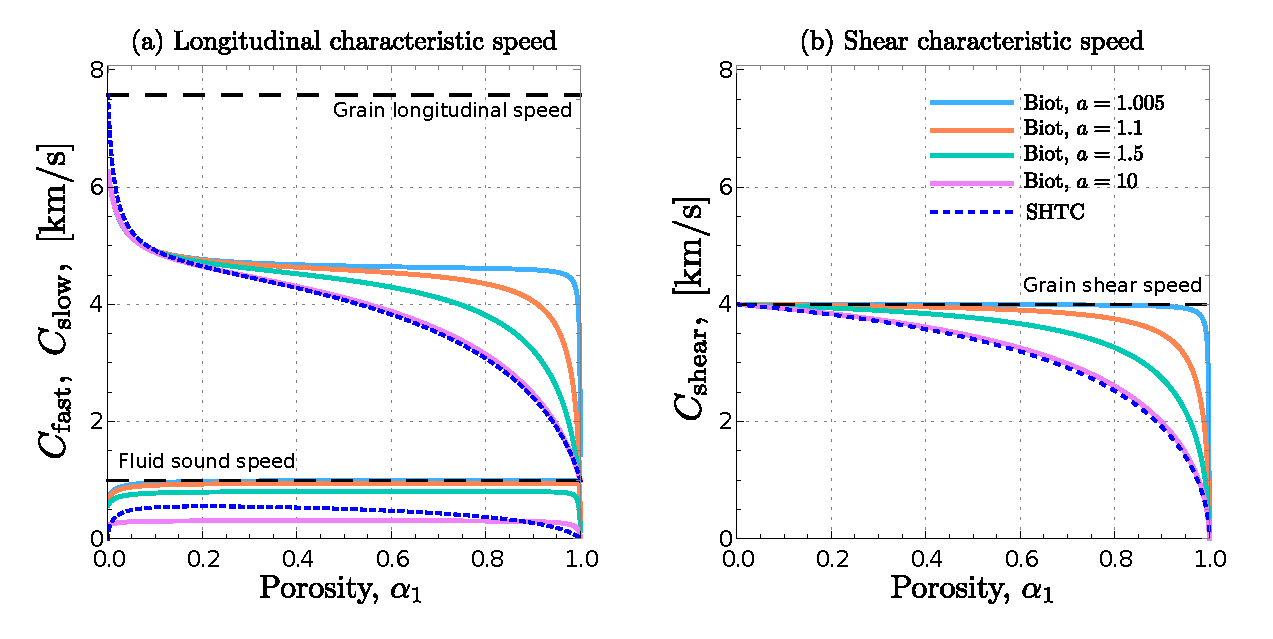
\includegraphics[draft=false,width=0.70\textwidth]{Figures/Biot_SHTC_speeds_porosity}
	\end{center}
	\vspace{-8mm}
	\caption{{\footnotesize \it Comparison of the characteristic speeds for the SHTC and Biot model 
	for different values of the tortuosity $ a $, (a): longitudinal fast and slow speeds, (b): 
	shear speeds.}}
	\label{fig1}
\end{figure}


\subsection{Dispersion relations and sound speeds}

\section{Numerical test problems for small amplitude wave propagation}


\begin{thebibliography}{}

	
\bibitem{Dorovsky}
Blokhin A.M., Dorovsky V. N., Mathematical Modelling in the Theory of Multivelocity Continuum, Nova Science Publishers, New York, 1995
	
\bibitem{Dumbser2016}
Michael Dumbser, Ilya Peshkov, Evgeniy Romenski, Olindo Zanotti,
High order ADER schemes for a unified first order hyperbolic formulation of continuum mechanics: Viscous heat-conducting fluids and elastic solids,
Journal of Computational Physics,
Volume 314,
2016,
Pages 824-862

\bibitem{Romenski2010}
Romenski E, Drikakis D, Toro E.F. Conservative models and numerical methods for one-dimensional compressible two-phase flow. \emph{J. Sci. Comp.} 2010; \textbf{42}:68.
	
\bibitem{Romenski2015}
Romenski E., Belozerov A. A., Peshkov I. M. Conservative Formulation for
Compressible Multiphase Flow. \emph{Quart. Appl. Math.} 2015. \textbf{74}. P. 113–136.

\bibitem{Peshkov2015}
Ilya Peshkov, Miroslav Grmela, Evgeniy Romenski, Irreversible mechanics and thermodynamics of two-phase continua experiencing stress-induced solid–fluid transitions \emph{Continuum Mech. Thermodyn.} (2015) 27:905–940, DOI 10.1007/s00161-014-0386-1

\bibitem{Wilmanski1998}
Wilmanski K. A thermodynamic model of compressible porous
materials with the balance equation of porosity. Transp Porous
Media 1998;32:21–47.

\bibitem{Wilmanski2003}
Wilmanski K. On thermodynamics of nonlinear poroelastic materials.
J Elast 2003;71:247–61.

\bibitem{Wilmanski2006}
Wilmanski K. A few remarks on Biot’s model and linear acoustics of poroelastic saturated materials.
\emph{Soil Dynamics and Earthquake Engineering} 2006; \textbf{26}. P. 509–536.

\bibitem{Khoei2011}
A.R. Khoei, T. Mohammadnejad
Numerical modeling of multiphase fluid flow in deforming porous media:
A comparison between two- and three-phase models for seismic analysis
of earth and rockfill dams. \emph{Computers and Geotechnics} 38 (2011) 142–166

\bibitem{Rohan2017}
Eduard Rohan, Vladimir Lukes.
Modeling large-deforming fluid-saturated porous media using an Eulerian incremental formulation.
Advances in Engineering Software, 
Volume 113, November 2017, Pages 84-95


\bibitem{Pesavento2017}
Francesco Pesavento, Bernhard A. Schrefler, Giuseppe Sciume.
Multiphase Flow in Deforming Porous Media: A Review.
Arch Computat Methods Eng (2017) 24:423–448

\bibitem{Merxhani2016}
Andy An introduction to linear poroelasticity. An introduction to linear poroelasticity.
arXiv:1607.04274v1 [physics.geo-ph] 14 Jul 2016.

\end{thebibliography}{}

\end{document}
	
	\bibitem{Ishii1975}
	Ishii M. \emph{Thermo-fluid dynamic theory of two-phase flow}. Eyrolles, Paris, 1975.
	
	\bibitem{Stewart1984} 
	Stewart BH, Wendroff B. Two-phase flow: models and methods. \emph{J. Comp. Phys.} 1984; \textbf{56}:363.
	
	\bibitem{Staedke2005}
	Staedke H, Francello G, et al. Advanced three-dimensional flow simulation tools for application to reactor safety (ASTAR).
	\emph{Nuclear Engineering and Design} 2005; \textbf{235}:379.
	
	\bibitem{Baer1986}
	Baer M, Nunziato J. A two-phase mixture theory for the deflagration-to-detonation transition (DDT) in reactive granular materials.
	\emph{Int. J. Multiphase Flow} 1986; \textbf{12}:861.
	
	\bibitem{Saurel1999}
	Saurel R, Abgrall R. A multiphase Godunov method for compressible multi-fluid and multiphase flows.
	\emph{J. Comput. Phys.} 1999; \textbf{150}:425.
	
	\bibitem{LeMetayer2005}
	Le~Metayer O, Massoni J, Saurel R. Modelling evaporation fronts with reactive Riemann solvers. \emph{J. Comput. Phys.} 2005; \textbf{205}:567.
	
	\bibitem{Kreeft&Koren2010}
	Kreeft JJ, Koren B. A new formulation of Kapila's
	five-equation model for compressible two-fluid flow, and its
	numerical treatment, {\it J. Comput. Phys.} 2010, \textbf{229}:6220.
	
	\bibitem{Zein2010}
	Zein A, Hantke M, Warnecke G. Modeling phase transition for
	compressible two-phase flows applied to metastable liquids,
	\emph{J. Comput. Phys.} 2010; \textbf{229}:2964.
	
	\bibitem{Herard2007}
	Herard JM. A Three-Phase Flow Model. \emph{Math. Comput.
		Modelling} 2007; \textbf{45}:732.
	
	\bibitem{Abgrall}
	
	Abgrall R, Saurel R. Discrete equations for physical and numerical compressible
	multiphase mixtures. {\it J. Comput. Phys.} 2003, \textbf{186}:361.
	
	\bibitem{Romenski2001}
	Romensky E. Thermodynamics and hyperbolic systems of balance
	laws in continuum mechanics. In \emph{Godunov Methods: theory
		and applications}, Toro EF. (ed). Kluwer Academic/Plenum
	Publishers, NY, 2001.
	
	\bibitem{Godunov2003}
	Godunov SK, Romenski E. \emph{Elements of continuum mechanics and conservation laws}, Kluwer Academic/Plenum Publishers, NY, 2003.
	
	\bibitem{Muller1998}
	Muller I, Ruggeri T. \emph{Rational extended thermodynamics}, Springer-Verlag, NY, 1998.
	
	
	\bibitem{Romenski2004}
	Romenski E, Toro EF. Compressible two-phase flows: two-pressure models and numerical methods. \emph{Computational Fluid Dynamics J.} 2004; \textbf{13}:403.
	
	\bibitem{Romenski2007}
	Romenski E, Resnyansky AD, Toro EF. Conservative hyperbolic model for compressible two-phase flow with different phase pressures and temperatures. \emph{Quarterly Applied Math.} 2007; \textbf{65}:259.
	
	\bibitem{Romenski2010}
	Romenski E, Drikakis D, Toro EF. Conservative models and numerical methods for one-dimensional compressible two-phase flow. \emph{J. Sci. Comp.} 2010; \textbf{42}:68.
	
	\bibitem{Mattia}
	La~Spina G, De'Michieli~Vitturi M. High resolution finite volume central schemes for a compressibile two-phase model, \emph{SIAM J. Sci. Comp.} 2012; \textbf{34}: B861. 
	
	\bibitem{Romenski2012_It}
	De'Michieli~Vitturi M, La~Spina G, Romenski E. 
	A compressible single temperature conservative two-phase model with phase
	transitions. in \emph{Numerical Analysis and
		Applied Mathematics ICNAAM 2013}, Simos TE, Psihoyios G, Tsitouras Ch (eds),
	AIP Conf. Proc.; \textbf{1558}:112, American Institute of Physics, NY, 2013.
	
	
	\bibitem{Zeidan2011}
	Zeidan D. On a further work of two-phase mixture conservation laws.
	in \emph{Numerical Analysis and Applied Mathematics ICNAAM 2011}, Simos TE, Psihoyios G, Tsitouras Ch, Zacharias Anastassi (eds),  AIP Conf. Proc.; \textbf{1389}:163, American Institute of Physics, NY,   2011.
	
	
	\bibitem{Romenski2012}
	Romenski E. Hyperbolic systems of conservation laws for
	compressible multiphase flows based on thermodynamically
	compatible systems theory, in \emph{Numerical Analysis and
		Applied Mathematics ICNAAM 2012}, Simos TE, Psihoyios G, Tsitouras Ch, Zacharias Anastassi (eds), AIP Conf. Proc. \textbf{1479}:62, American Institute of Physics, NY, 2012.
	
	\bibitem{ToroBook}
	{Toro EF.}  \textit{Riemann solvers and numerical methods in
		fluid dynamics} Springer-Verlag, Second Edition,1999.
	
	\bibitem{friedrichs1954}
	{Friedrichs KO.} {Symmetric hyperbolic linear differential
		equations}. \textit{Comm. Pure Appl. Math.} 1954; {\bf 7}: 
	345.
	
	\bibitem{ToroTitarev}
	{Toro EF, Titarev VA.}  {MUSTA schemes for systems of
		conservation laws}, {\it J. Comput. Phys.}2006 \textbf{216}: 403.
	
\end{thebibliography}{}